\newpage
\chapter{System Design}
\clearpage
\section{System Architecture}
{\normalsize{The system architecture diagram represents a high level model of the whole project showcasing the important modules of the program. The request for translation for the audio originated from the user, which would be done by the user interface and the designed API. This request is then transmitted to the server where, it is first of all validated by server and further will be processed through the three models, i.e., the speech synthesizer, the translator model, and finally by the text to speech synthesizer. This after successful processing is transmitted back to the user, where is able to hear the audio is in the desired language.}}


\begin{figure}[h]
  \begin{center}
\tcbox{  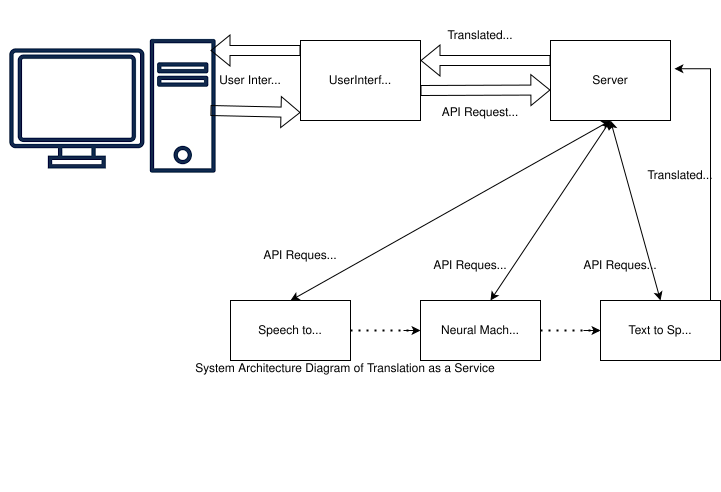
\includegraphics[height=90mm]{Images/Figures/System Architecture.png}}
  \caption{System Architecture}
  \end{center}
\end{figure}

\vspace*{0.2cm}
\newpage

\clearpage
\section{Data Flow Diagrams}
\subsection{DFD Level 0}
{\normalsize{The DFD Level 0 diagram show case the abstract view of the project, where the user shall be providing the audio source and then receive a translated audio output in the desired language.}}
\newline
\newline
\begin{figure}[h]
  \begin{center}
  \tcbox{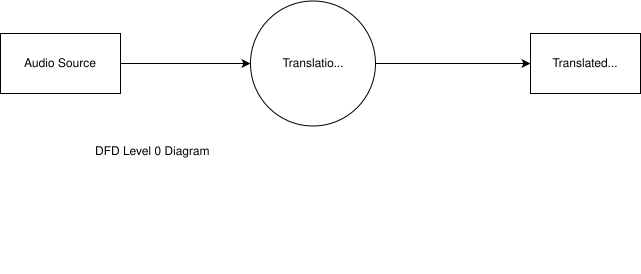
\includegraphics[height=60mm]{Images/Figures/DFD(Level 0).drawio (1) (1).png}}
  \caption{DFD Level 0}
  \end{center}
\end{figure}

\clearpage
\subsection{DFD Level 1}
{\normalsize{The Level 1 diagram, represents the module where the software resides and how the server interacts with the model for translation.}}
\newline
\newline
\begin{figure}[h]
  \begin{center}
  \tcbox{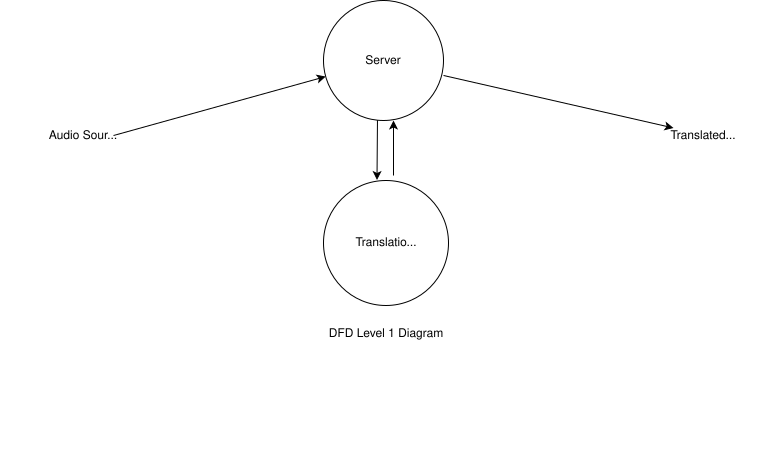
\includegraphics[height=80mm]{Images/Figures/DFD(Level 1).png}}
  \caption{DFD Level 1}
  \end{center}
\end{figure}
\newpage

\clearpage
\subsection{DFD Level 2}
{\normalsize{The DFD Level 2 represents each module present at the server and how the data is being processed from one to another. It has three models, the speech to text synthesizer, the translator, and the text to speech synthesizer.}}
\newline
\newline
\begin{figure}[h]
  \begin{center}
\tcbox{  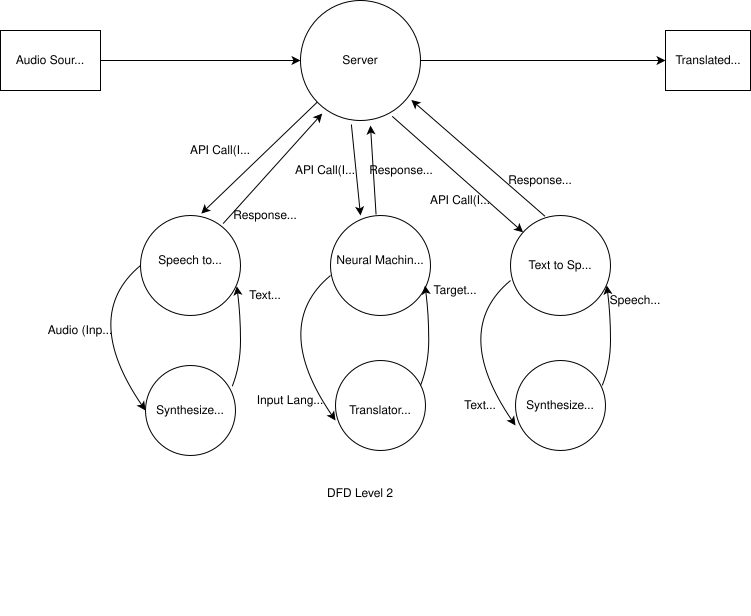
\includegraphics[height=100mm]{Images/Figures/DFD(Level2) (1).png}}
  \caption{DFD Level 2}
  \end{center}
\end{figure}

\clearpage
\section{UML Diagrams}
\subsection{Use Case Diagram}
{\normalsize{The use case diagram shows how the all actors, i.e., user and system interact with each other to make the translation successful.
\newline
The user request through the user interface by providing the appropriate input data, audio source. The server is sent a. API request for the translation. The server initiates the required sequences, and checking all the interaction and transmissions are working appropriately. The system provides the services to carry out the translation.
}}
\newline
\newline
\begin{figure}[h]
  \begin{center}
  \tcbox{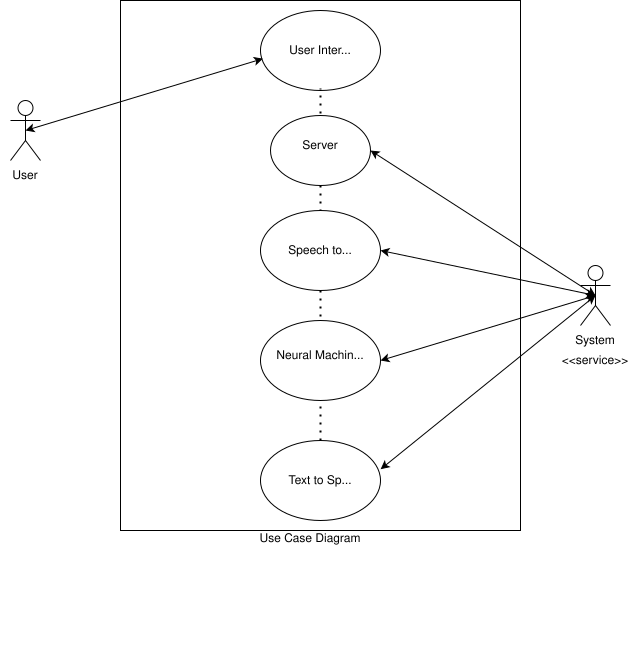
\includegraphics[height=80mm]{Images/Figures/Use Case Diagram.png}}
  \caption{Use Case Diagram}
  \end{center}
\end{figure}

\clearpage
\subsection{Activity Diagram}
{\normalsize{The activity diagram show case all the activities that occur from initialing the sever with the deployed model, to the successful interaction and translation of the audio into the desired language.
\\
In this first the server is initiated with the model deployed in it, and it checks for the status of the server. If the status is in working state, then further actions are proceeded. Otherwise, it checks for the status until it gets activated. Then the server listens for the request for services.
\\
The user starts the application section, and the connection with the server is established, for the further services. After that the user send the input data, i.e., the audio file, along with the current language and the desired language names. \\
The server then listens to the requests and check if it is a valid request and the inputs are in appropriate format. If it is valid request then further processing is done. Otherwise, error message is displayed and the server again listens for the request and data. \\
The server then transmits the request to the three models sequentially, along with checks for any error. At each stage the data is processed and transformed in the desired format.\\
Finally, if all the stages proceed without any error, then the audio file is provided as output the user, in the desired language. \\ 
The request session interaction goes on until, the user terminates the session. \\ 
}}
\newline
\newline
\begin{figure}[h]
  \begin{center}
 \tcbox{ 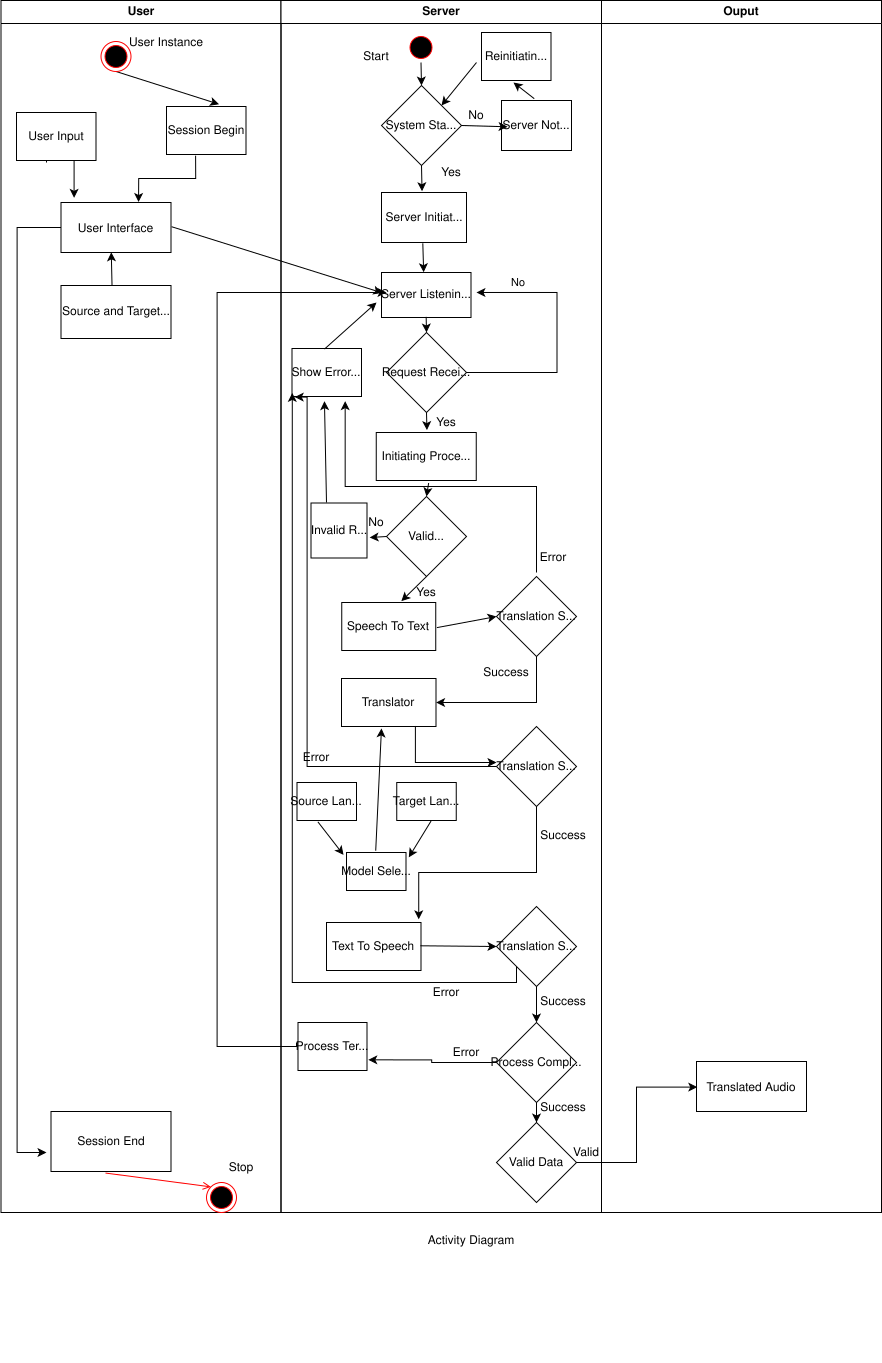
\includegraphics[height=210mm]{Images/Figures/Activity Diagram.png}}
  \caption{Activity Diagram}
  \end{center}
\end{figure}


\clearpage
\subsection{Sequence Diagram}
{\normalsize{Sequence diagram show the interaction of the user and the server, along with the session duration and all the actions that occur between them. \\ 
The session request to the server last from sending the input data to server for processing to the translated output received at the user end. \\
}}
\newline
\begin{figure}[h]
  \begin{center}
  \tcbox{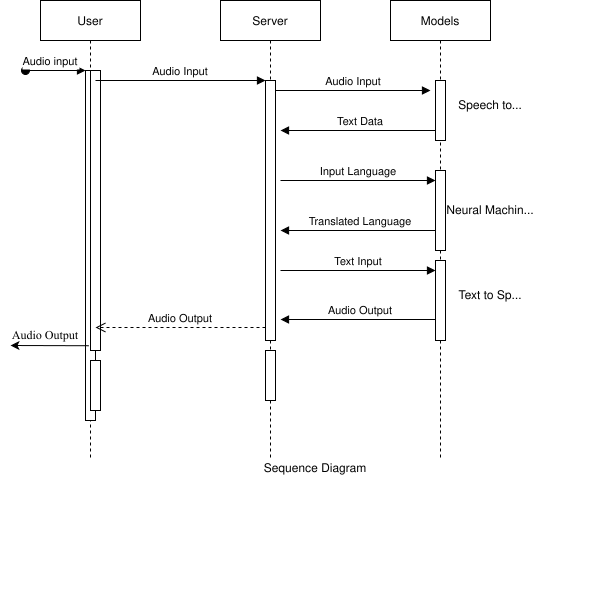
\includegraphics[height=120mm]{Images/Figures/Sequence Diagram1.png}}
  \caption{Sequence Diagram}
  \end{center}
\end{figure}

\clearpage
\subsection{Class Diagram}
\newline
\begin{figure}[h]
  \begin{center}
  \tcbox{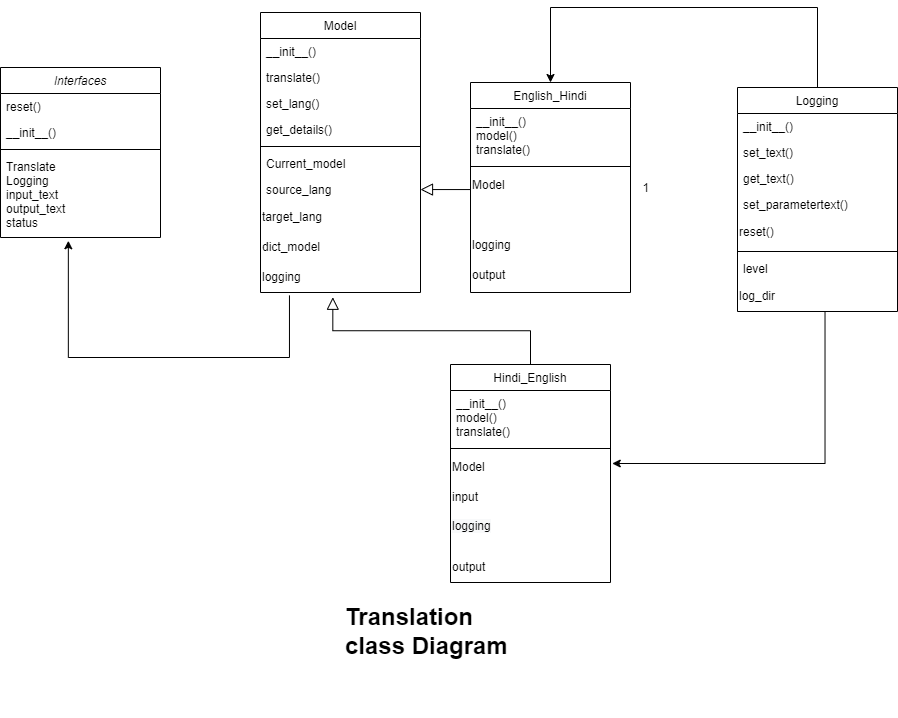
\includegraphics[height=120mm]{Images/Figures/Class_Diagram.png}}
  \caption{Class Diagram}
  \end{center}
\end{figure}
